\section{Fine-Grained Static Mechanisms for Extreme-Token Phenomena} \label{sec:circuit}

In this section, we will identify more fine-grained static mechanisms for extreme-token phenomena in Llama 3.1-8B-Base. To do this, we identify circuits for the origin of attention sinks and small value states. Then, using ablation studies, we study the origin of massive norms. Again, we use the generic test phrase ``\bos{} Summer is warm. Winter is cold.''

\begin{figure}[h]
    \centering
    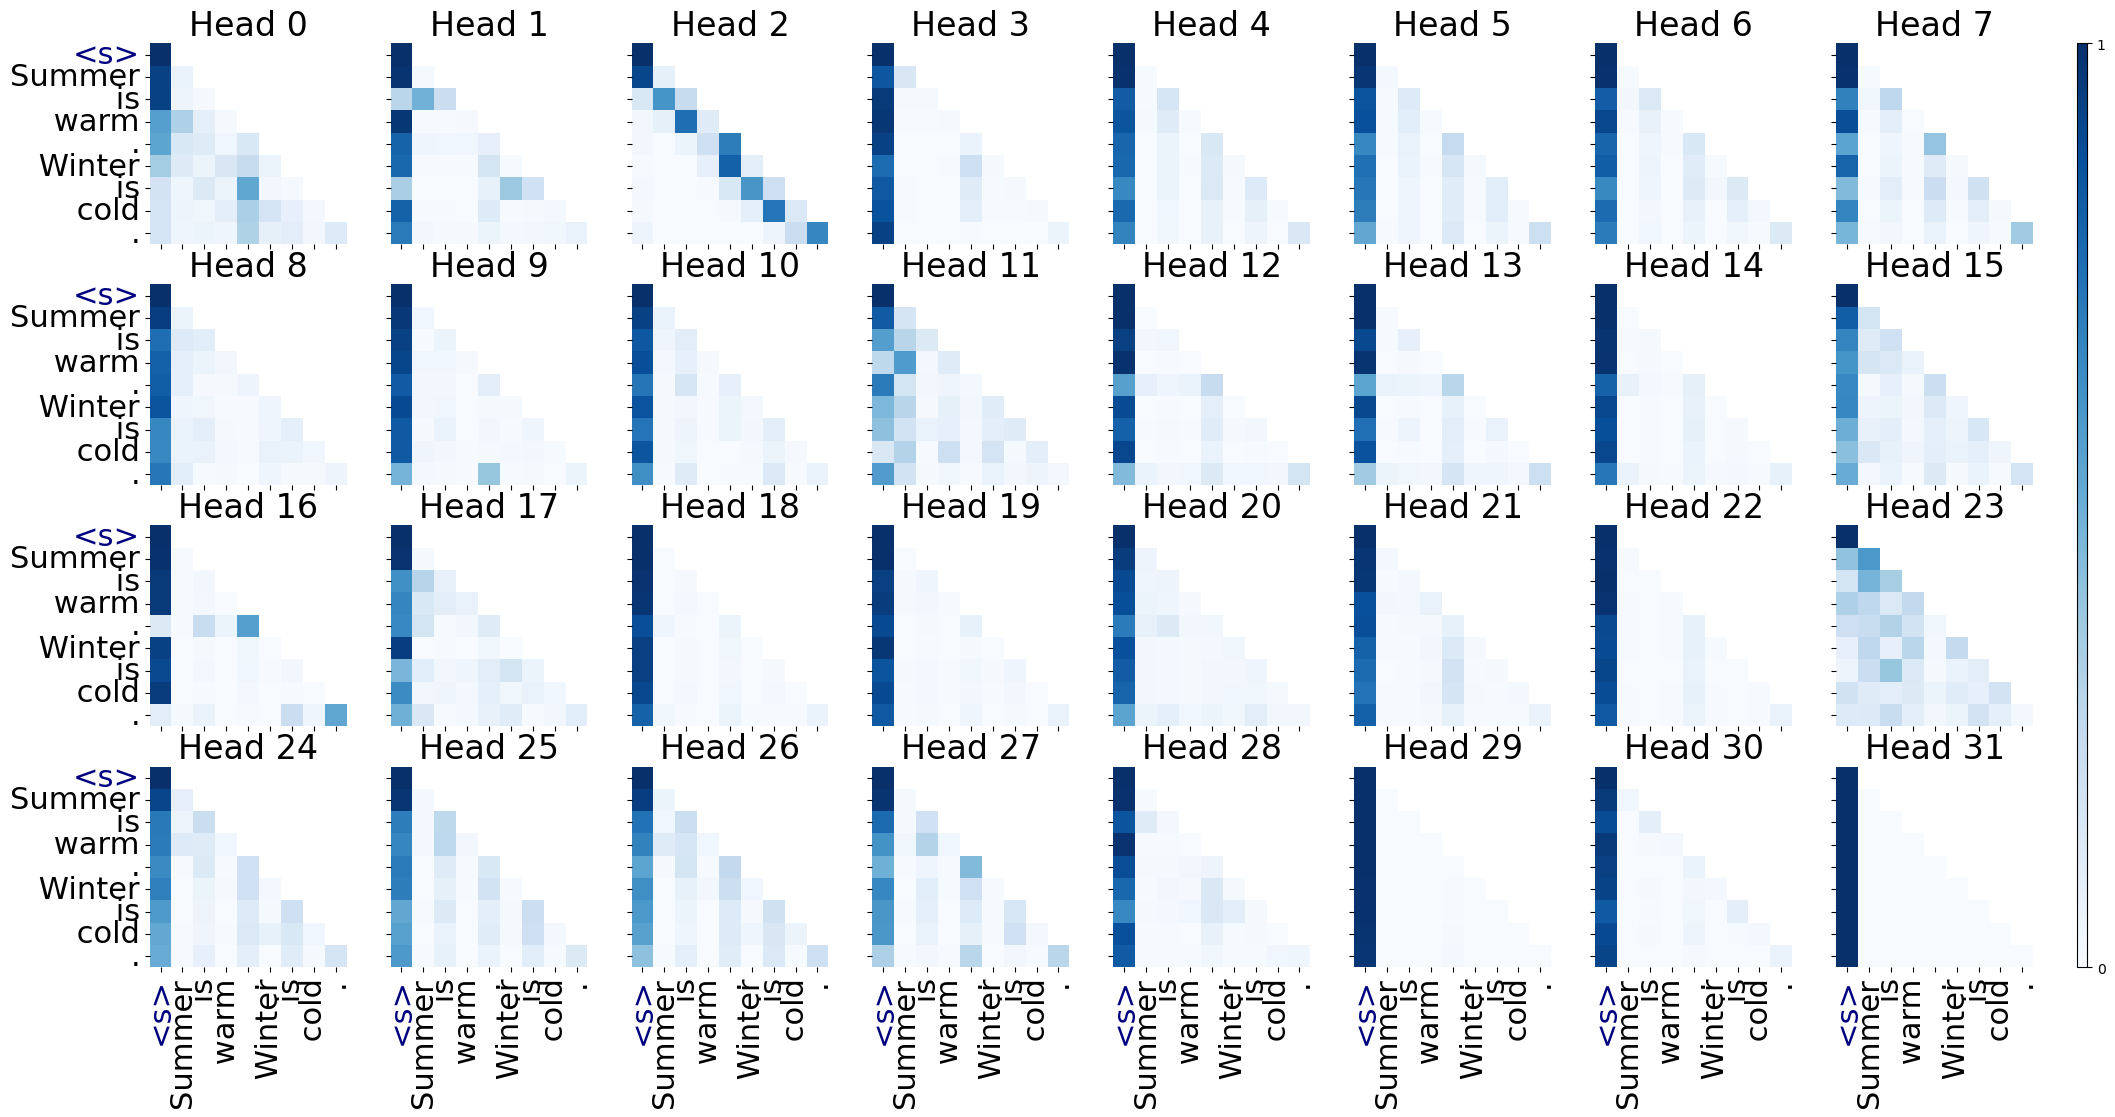
\includegraphics[width=\textwidth]{Figures/llama_31_circuit/llama_31_attn_l0.png}
    \caption{\small \textbf{A visualization of attention heads at Layer 0 of Llama 3.1-8B-Base.} Notice that many heads have the attention sink property, even at Layer 0 without any cross-token interaction. As usual, the test phrase is ``Summer is warm. Winter is cold.'' The most clear attention sink is Head 31.}
    \label{fig:llama_31_attn_layer0}
\end{figure}

\begin{figure}[h]
    \centering
    \begin{subfigure}[t]{0.49\textwidth}
    \caption{Alignment of query states and key states (L0H31).}
        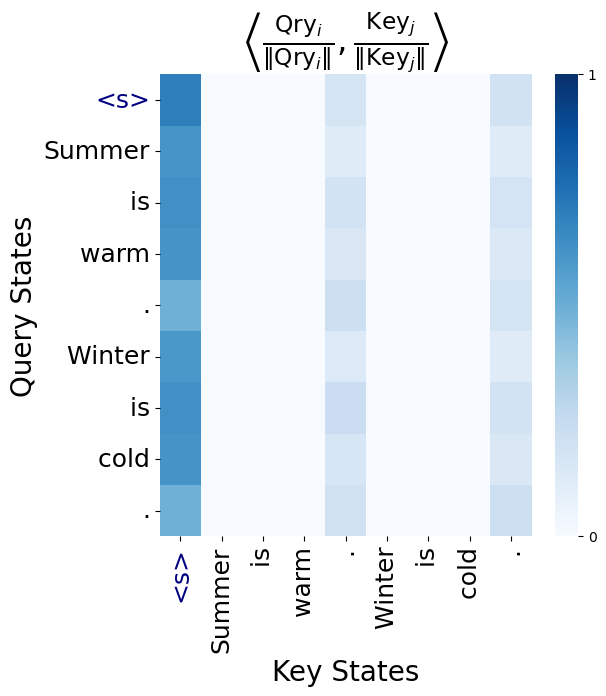
\includegraphics[width=\textwidth]{Figures/llama_31_circuit/llama_31_qk_l0.png}
    \end{subfigure}
    \hfill
    \begin{subfigure}[t]{0.49\textwidth}
        \caption{Alignment of key states and key states (L0H31).}
        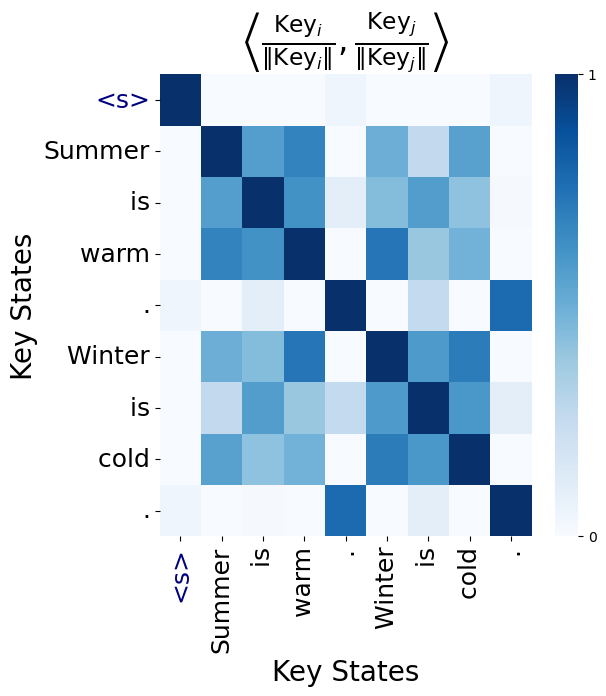
\includegraphics[width=\textwidth]{Figures/llama_31_circuit/llama_31_kk_l0.png}
    \end{subfigure}
    \caption{\small \textbf{Alignment between query states and key states at Layer 0 Head 31 of Llama 3.1-8B-Base.} We observe that the key state of \bos{} is orthogonal to all other key states, and heavily aligned with all query states. Meanwhile, all semantically meaningful (i.e., not delimiter) tokens have aligned key states.}
    \label{fig:llama_31_qk_kk}
\end{figure}

\paragraph{Attention sinks and global contextual semantics.} There are many attention sinks at layer \(0\), and the \bos{} token is always the sink token (see \Cref{fig:llama_31_attn_layer0}). From now on until the end of this section, we \textit{restrict our attention to Head 31 of Layer 0, which is an attention sink.} These attention sinks are caused by two linear-algebraic factors, demonstrated in \Cref{fig:llama_31_qk_kk}.
\begin{enumerate}
    \item The key state of the \bos{} token has small dot product with all other tokens. 
    \item The query states of all tokens are nearly orthogonal to the key states of all tokens except the \bos{} token.
\end{enumerate}
 These two facts combine to ensure that the key state of the \bos{} token is picked out by each query state, causing the attention sink. Since these query and key states are produced without any cross-token interaction, the alignment of different states is caused purely by the token's global importance or meaning imparted via pretraining. The \bos{} token has no semantic meaning in the context of prose tokens, so its key state is not aligned with key states of meaningful prose tokens. Also, delimiter tokens, oft considered secondary attention sinks (c.f.~\Cref{sub:fixed_bos}), have the most aligned key states to the key state of the \bos{} token, and are also the tokens with the least semantic meaning in the prose context. Thus, we identify that, at least in this restricted example, query state and key state alignment depends heavily on the contextual semantics of the token.

 \begin{figure}[h]
     \centering
     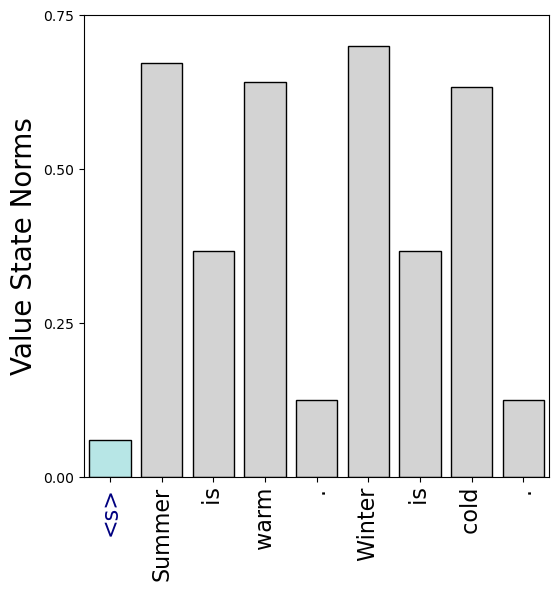
\includegraphics[width=0.4\linewidth]{Figures/llama_31_circuit/llama_31_value_states.png}
     \caption{\small \textbf{Value state drains at Layer 0 Head 31 of Llama 3.1-8B-Base.} We observe that the value state associated with \bos{} is already much smaller than every other semantically meaningful token, and still smaller than the delimiter tokens in the same sentence.}
     \label{fig:llama_31_value_states}
 \end{figure}

\paragraph{Value state drains.} The value states of the \bos{} token at Layer \(0\) Head 31 are already near zero, as demonstrated in \Cref{fig:llama_31_value_states}. While the delimiter tokens, which are less semantically meaningful in the prose context, have smaller value states than the rest, they are not as small as the value state of the \bos{} token which is guaranteed to not have any semantics.

\begin{figure}[h]
    \centering
    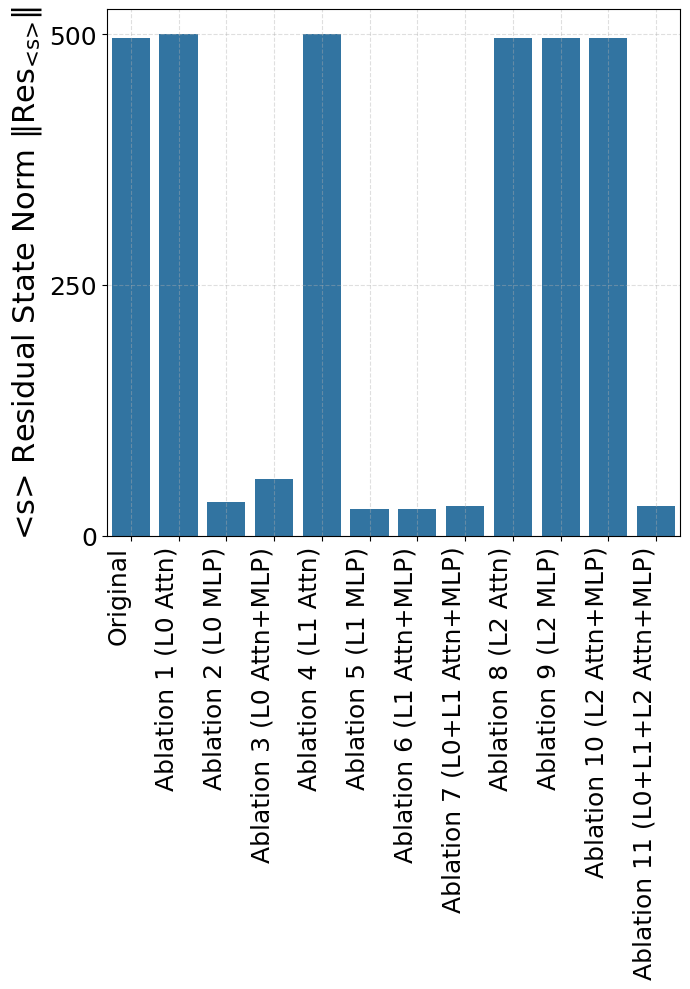
\includegraphics[width=0.5\textwidth]{Figures/llama_31_circuit/llama_31_massive_norms.png}
    \caption{\small\textbf{Ablation study on the cause of the residual state peak in Llama 3.1-8B-Base.} We perform a series of ablations to understand which components of the network promote the residual state peaks. We find that ablating either the zeroth or first layer's MLP is sufficient to remove the residual state peak phenomenon, while no other layer-level ablation can do it.}
    \label{fig:enter-label}
\end{figure}

\paragraph{Residual state peaks.} Residual state peaks are caused by the first two layers' MLPs. In particular, we perform several ablations, comparing between the residual state norms in a later layer (\(24\)) of an un-edited forward pass versus forward passes where we force the output of either multiple layers, a single layer, an attention block, or an MLP to be zero (and hence remove its contribution from the residual stream). This intervention showed that ablating \textit{either} Layer 0's or Layer 1's MLP is sufficient to remove the residual state peak. In particular, the second-largest token at Layer 24 in \textit{each} ablation (including the original setup) has norm between \(29\) and \(38\), so the interventions ensure that all tokens have similar size.

% \begin{figure}
%     \centering
%     \begin{subfigure}[t]{0.24\textwidth}
%         \centering 
%         \caption{\small Attention sinks (L0).}
%         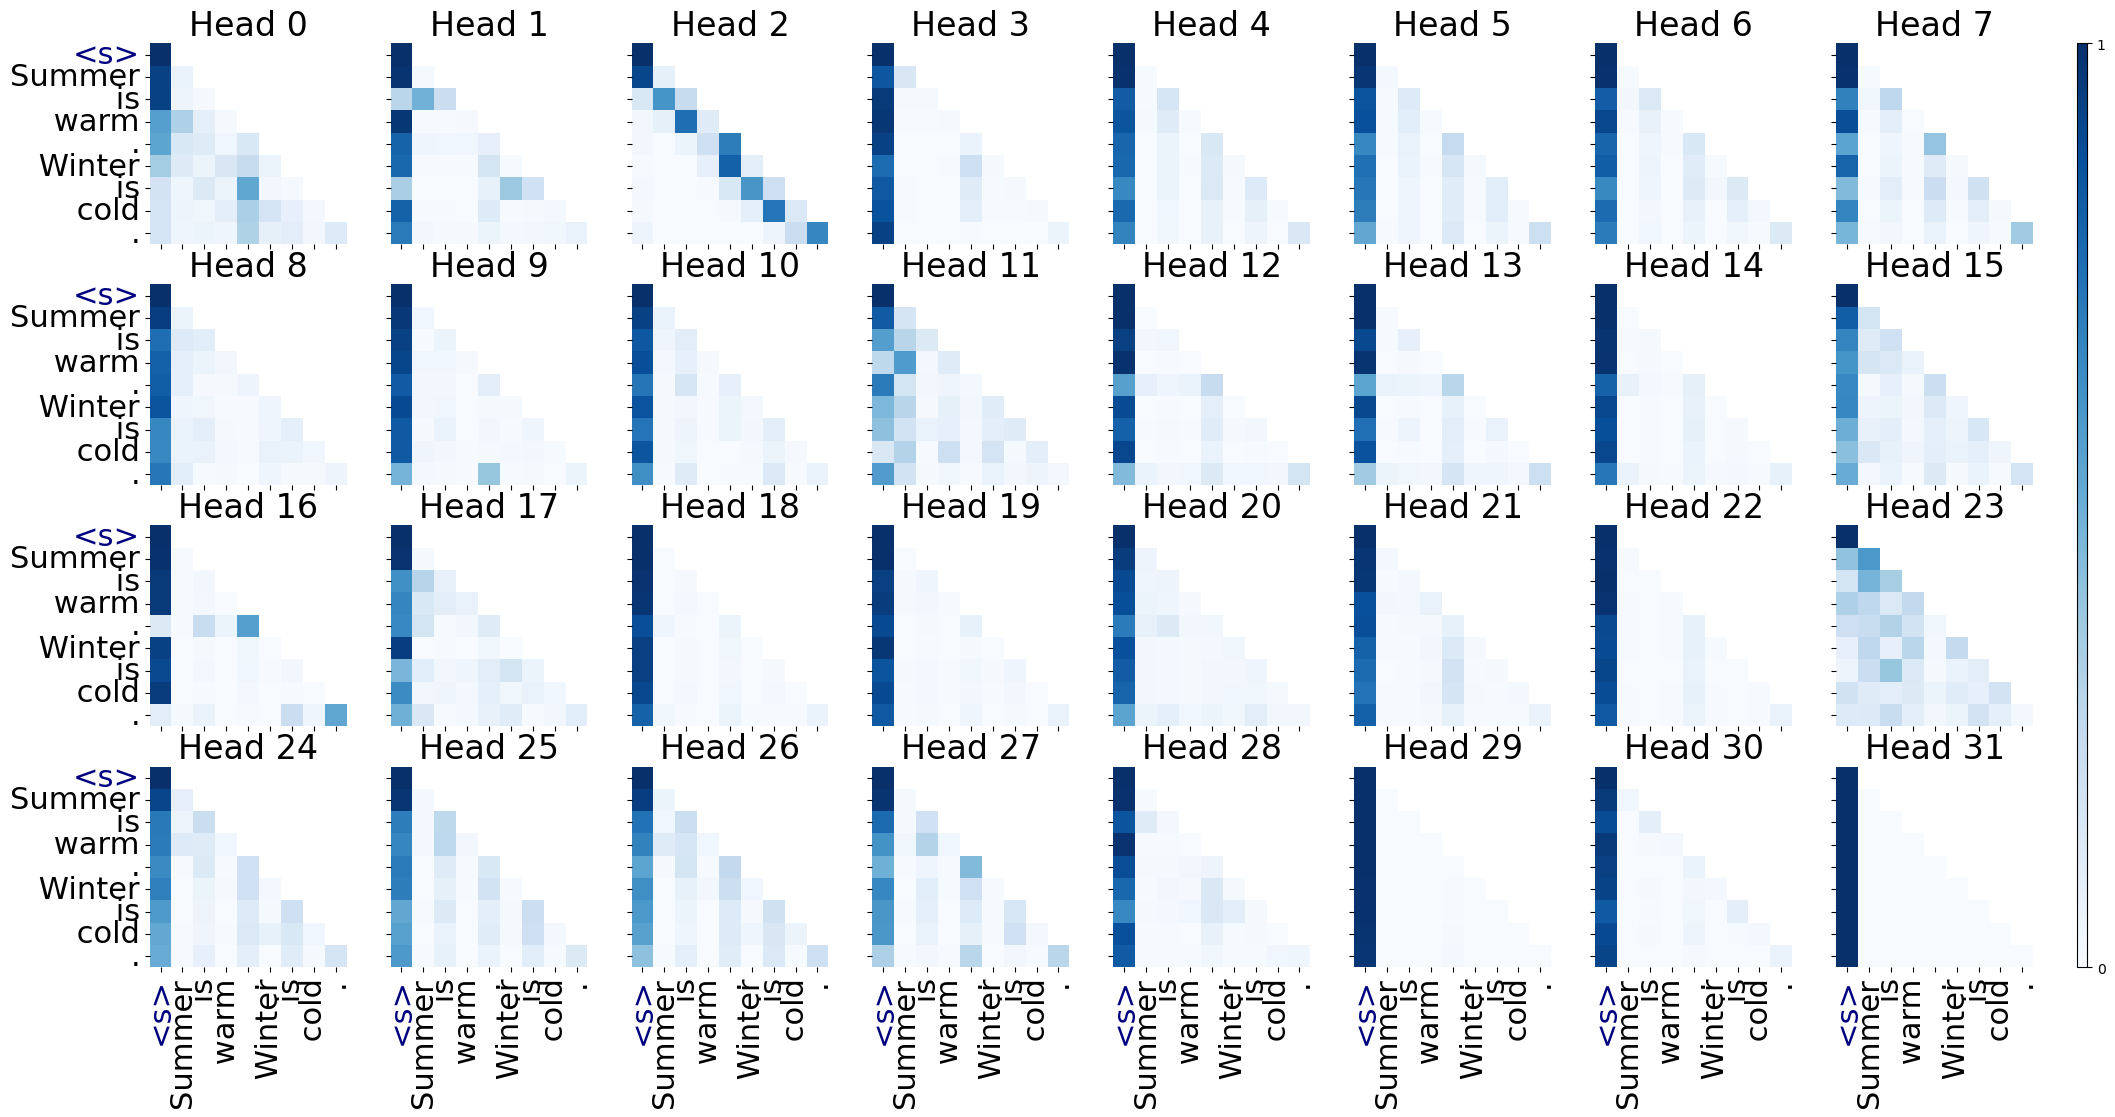
\includegraphics[width=\textwidth]{Figures/llama_31_circuit/llama_31_attn_l0.png}
%         \label{fig:llama_31_attn_sink_l0}
%     \end{subfigure}
%     \begin{subfigure}[t]{0.32\textwidth}
%         \centering 
%         \caption{\small Value norms (L0H31).}
%         \includegraphics[width=\textwidth]{Figures/llama_31_circuit/llama_31_value_l0.png}
%         \label{fig:llama_31_v_l0}
%     \end{subfigure}
%     \begin{subfigure}[t]{0.49\textwidth}
%         \centering 
%         \caption{\small Correlations between query/key states (L0H31).}
%         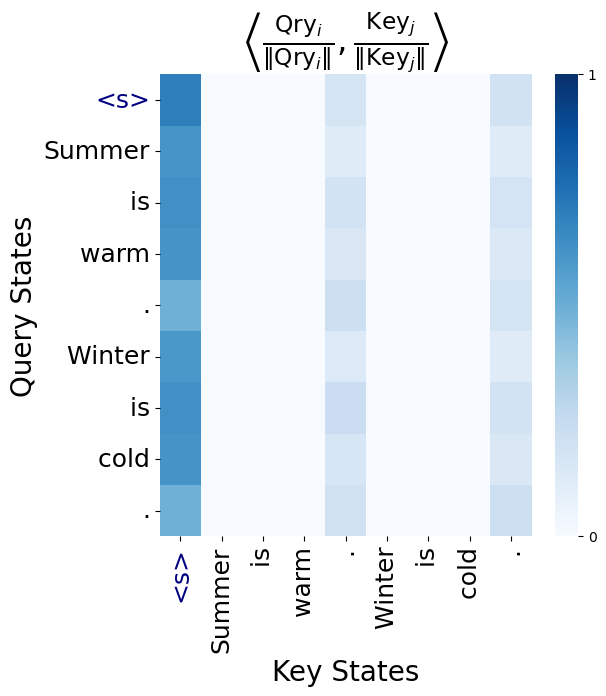
\includegraphics[width=0.49\textwidth]{Figures/llama_31_circuit/llama_31_qk_l0.png}
%         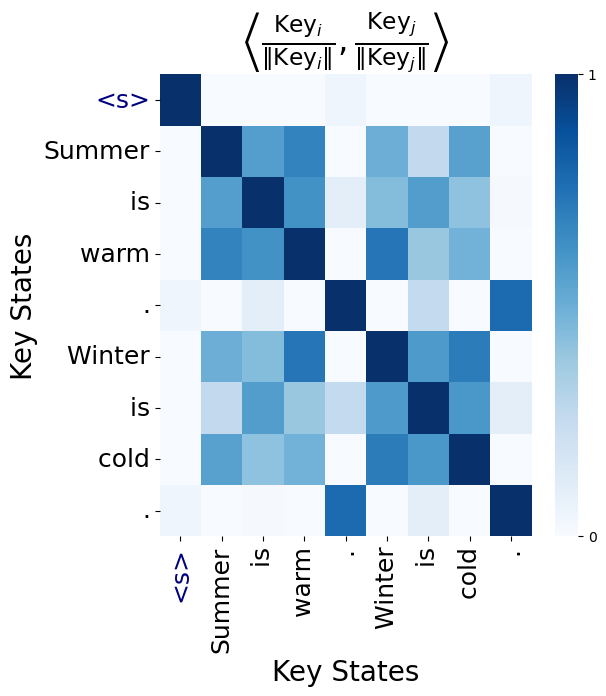
\includegraphics[width=0.49\textwidth]{Figures/llama_31_circuit/llama_31_kk_l0.png}
%         \label{fig:llama_31_qk_kk_l0}
%     \end{subfigure}
%     \begin{subfigure}[t]{0.24\textwidth}
%         \centering 
%         \caption{\small Res.~stream ablations.}
%         \includegraphics[width=\textwidth]{Figures/llama_31_circuit/llama_31_massive_norm.png}
%         \label{fig:llama_31_resid_l0}
%     \end{subfigure}
    
%     %\includegraphics[width=0.5\linewidth]{}
%     \caption{\small \textbf{A circuit for extreme-token phenomena in Llama 3.1-8B-Base.} \textit{Top:} Attention sinks present in Layer 0. \textit{Left:} Value states of tokens which are semantically irrelevant for prose are small, and the \bos{} token (which is always semantically irrelevant) is the smallest. Since these value states are in the zeroth layer, they have not been computed via any cross-token interaction, so this is a result about how tokens align with the value weight matrix as per their usefulness. \textit{Middle:} In the first layer, attention sinks form because key states of semantically irrelevant tokens are correlated with all query states, while other key states are nearly orthogonal to all query states. Meanwhile, all semantically relevant key states are nearly orthogonal to semantically irrelevant key states, and are very aligned with each other. Again, the query and key states were computed in the zeroth layer and so without any previous cross-token interaction, so this shows how the zeroth-layer query and key weight matrices align to tokens depending on their semantic meaning as inferred by pre-training. \textit{Right:} Residual state peaks are present due to the MLPs in the first two layers: ablating either of them by manually removing their contribution to the residual stream is sufficient to remove the residual-state peaks, but ablating any other components will preserve the residual state peak phenomenon. % Evidence of a circuit for massive norm, attention sink, value states in Llama 3.1
%     %\DP{TODO: left figure is show a few attention heatmaps, like 4 or 8; middle figure is show Q dot K, K dot K, and value norms; right figure is residual norm}
%     }
%     \label{fig:llama_31_circuits}
% \end{figure}
